% !TeX root = ../main.tex

\section{Experiments}

% We evaluate \tool based on the following research questions.

Carlin et al.\cite{carlini2021extracting}. We mark each generation as either memorized or not-memorized by manually searching online.


LOSS\cite{yeom2018privacy}
ZLib\cite{carlini2021extracting}
Min-K\cite{shi2023detecting}
Gotcha\cite{yang2024gotcha}
DC-PDD\cite{}

% Main document content
\subsection{Setup}


\textbf{Baselines.} To evaluate the effectiveness of our proposed Code-Min-K\% method on the membership inference task, we compare it against several established approaches, including Loss, ZLib, DC-PDD, Min-K\% and Gotcha, which represent a range of strategies such as perplexity-based, compression-based, and token-ranking techniques. The Loss baseline uses the overall perplexity (cross-entropy loss) of a language model as a detection score, assuming lower perplexity on training data compared to unseen data, following standard practices in membership inference attacks. ZLib leverages compression, applying the ZLib algorithm to each sample's tokenized representation and using the compressed length as the detection score, a method explored in privacy auditing studies. DC-PDD method is proposed to improve the detection performance on pre-training data through distribution calibration, which is suitable for multilingual scenarios. Min-K\% ranks tokens by likelihood and uses the bottom K\% (ranging from 0.1 to 1.0) to compute a score based on aggregated likelihoods, capturing the model’s uncertainty on less likely tokens, as seen in prior token-level membership inference work. GOTCHA is a MIA approach to code completion models.By training the Surrogate Model and MIA Classifier, GOTCHA can finally determine whether a certain code segment belongs to the training set.

\textbf{Targeted LLMs.} The experiment evaluates four mainstream open-source language models, selected to represent diverse scales and architectures: \textit{EleutherAI/pythia-2.8b}, a 2.8B parameter Transformer model with strong code generation capabilities; \textit{EleutherAI/pythia-12b}, a 12B parameter Transformer model with improved reasoning and instruction-following abilities; \textit{EleutherAI/gpt-neo-2.7B}, a 2.7B parameter Transformer model designed for text generation and creative tasks; \textit{StabilityAI/stablelm-base-alpha-3b}, a 3B parameter model optimized for code generation and low-resource deployment. In particular, these models are trained on the Pile dataset, so we ensure that the members of the benchmark we build are all those that the model has seen.


\textbf{Metrics.} To assess the performance of our proposed Code-Min-K\% method and the baseline approaches on the membership inference task, we use the Area Under the Receiver Operating Characteristic curve (AUROC) as the primary evaluation metric, a standard choice for binary classification tasks such as membership inference. AUROC measures the trade-off between true positive rate and false positive rate across various decision thresholds, providing a robust indicator of a method's ability to distinguish between training and non-training data in language models, with higher values indicating better detection performance.

\textbf{Environment.} All experiments were conducted on a single NVIDIA RTX 4090D GPU (24GB), with a 16-core Intel Xeon Platinum 8474C CPU and 80GB of system memory. The software stack includes Ubuntu 20.04, Python 3.8, PyTorch 2.0.0, and CUDA 11.8.


\subsection{Results}

We systematically compare the AUROC performance of various detection methods on the membership inference task across four mainstream open-source language models, with results presented in Table~\ref{tab:main_results}. Overall, \textbf{Code-MiNK consistently outperforms the original methods and other baselines across all models and K-value settings}, demonstrating stable and widespread performance advantages.

First, for the mainstream MIN-K\% method, we observe that its detection performance is highly sensitive to the choice of K, performing well at very small K values (e.g., 0.1) but often degrading in other settings. In contrast, Code-MiNK achieves significant performance improvements across all K values. For instance, on Pythia-2.8B, the AUROC improves from 47.8\% to 56.3\%; on Phi-2, from 60.0\% to 51.9\%; on TinyLLaMA, from 37.1\% to 51.8\%; and on LLaMA-7B, from 38.5\% to 52.7\%.

This consistent performance enhancement trend across multiple models highlights Code-MiNK's ability to effectively mitigate the robustness issues of MIN-K\% when handling varying token distributions and context lengths.

Second, traditional compression-based metrics (e.g., ZLib) and overall perplexity metrics (e.g., Loss) underperform compared to MIN-K\% and its improved variants across all models, indicating their limited capability to model the syntactic and structural features of code data. For example, on LLaMA-7B, ZLib achieves an AUROC of only 31.0\%, significantly lower than Code-MiNK's best result of 52.7\%.

Furthermore, the consistent performance gains from large models (Pythia-12B) to lightweight models (GPT-Neo-2.7B) suggest that Code-MiNK offers strong architectural adaptability and scalability, making it suitable for deployment and transfer across diverse hardware resource constraints.

\begin{table}[!t] 
\centering
\caption{Comparison of methods across different models with AUROC scores (\%)}\label{tab:main_results}
\begin{tabular}{m{2cm}m{2.6cm}m{1.8cm}m{1.8cm}m{1.8cm}m{1.8cm}}
\toprule
\textbf{Language} &\textbf{Method} & \textbf{Pythia-2.8B} & \textbf{Pythia-12B} & \textbf{GPT-Neo-2.7B} & \textbf{StableLM-Alpha-3B}\\
\midrule

\multirow{6}{*}{Python} & Loss & 37.1 & 59.5 & 29.2 & 33.9 \\
&ZLib & 31.5 & 32.6 & 29.3 & 31.0 \\
&Min-K Prob & 39.2  & 57.9  & 31.2  & 34.4  \\ % K=0.2
&\textsc{Gotcha} & & & &\\
&\textsc{DC-PDD} & & & &\\\cmidrule{2-6}
&\tool-0.1 & 56.3 & 51.9  & 51.8 & 52.7  \\\hline

\multirow{6}{*}{Java} & Loss & 37.1 & 59.5 & 29.2 & 33.9 \\
&ZLib & 31.5 & 32.6 & 29.3 & 31.0 \\
&Min-K Prob & 39.2  & 57.9  & 31.2  & 34.4  \\ % K=0.2
&\textsc{Gotcha} & & & &\\
&\textsc{DC-PDD} & & & &\\\cmidrule{2-6}
&\tool-0.1 & 56.3 & 51.9  & 51.8 & 52.7  \\
\bottomrule
\end{tabular}
\end{table}






\begin{table}[!t] 
    \centering
    \caption{AUROC Score of \tool under Different Lengths}
    \begin{tabular}{m{2cm}m{2cm}m{1.8cm}m{1.8cm}m{1.8cm}m{1.8cm}}
    \toprule
    \textbf{Language} &\textbf{Length} & \textbf{Pythia-2.8B} & \textbf{Pythia-12B} & \textbf{GPT-Neo-2.7B} & \textbf{StableLM-Alpha-3B}\\
    \midrule
    \multirow{3}{*}{Python} & Short & & & & \\
     & Mid & & & & \\
    &High & & & & \\
    \hline
    \multirow{3}{*}{Java} & Short & & & & \\
     & Mid & & & & \\
    &High & & & & \\
    \bottomrule
    \end{tabular}
    \label{tab:main_results}
\end{table}

\subsection{Robustness}

\textbf{Model Size.}

\textbf{Function Length.}


\subsection{Ablation Study}

% ε


\textbf{\todo{Ablation on the external method calls.}}

\textbf{\todo{Ablation on the keywords.}}


\subsection{Parameter Analysis}

\textbf{AUROC w.r.t Hyperparameter k\%.}

\textbf{AUROC Curve.}



\begin{figure}[!t]
    \centering
    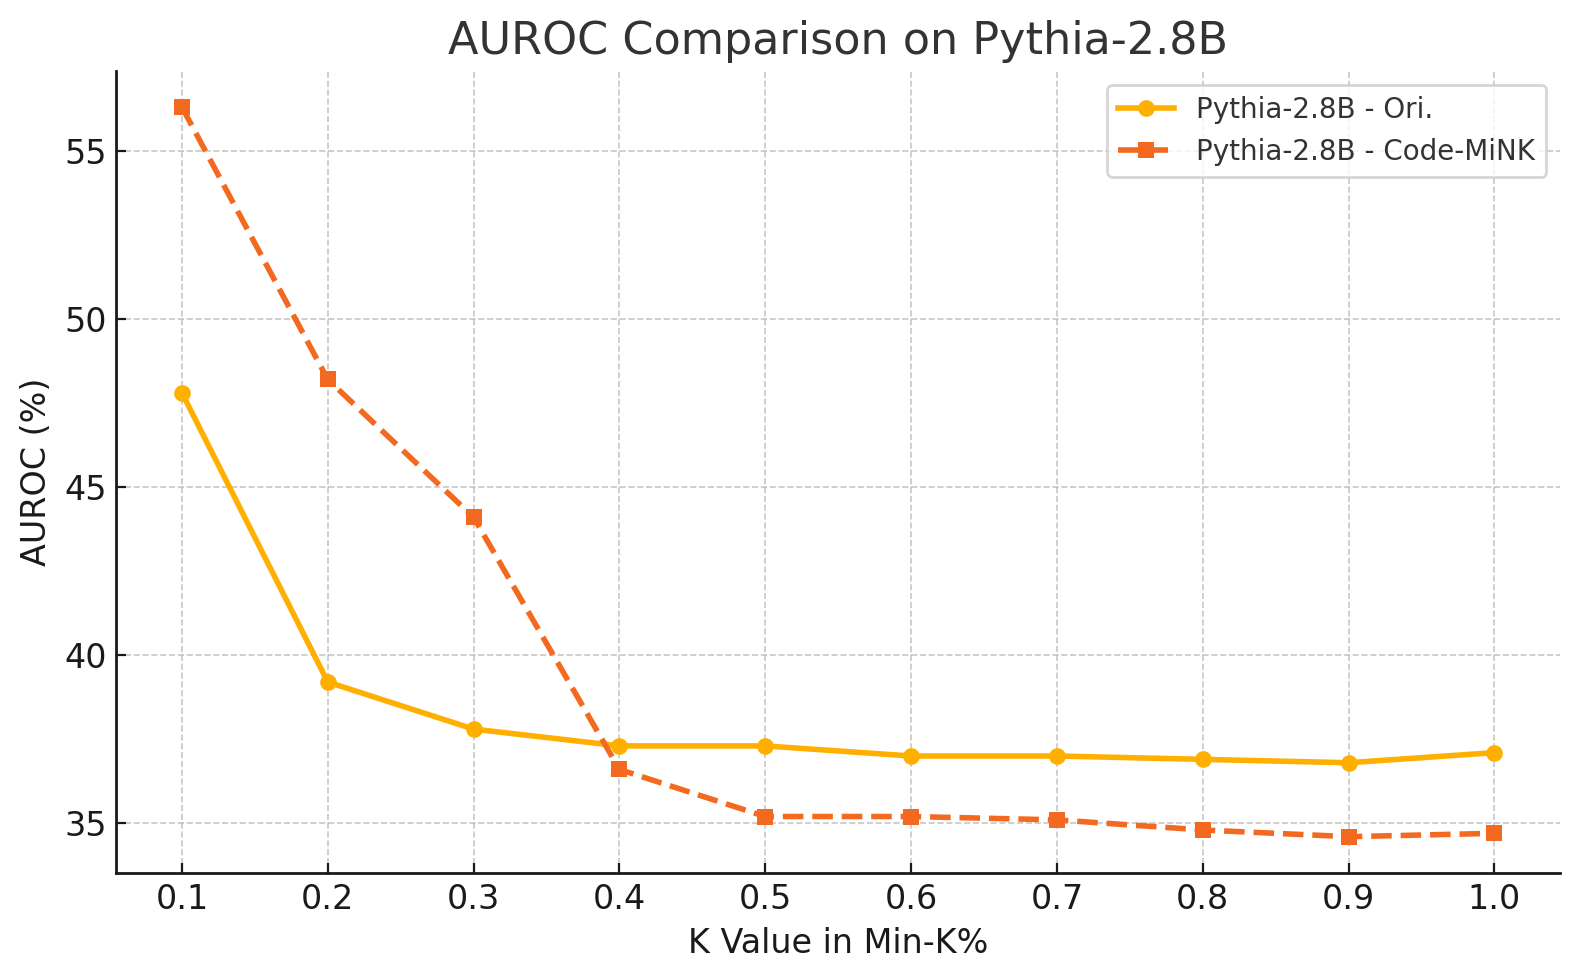
\includegraphics[width=0.7\textwidth]{./resource/pythia2_8b.png}
    \caption{AUROC performance under Hyperparameter K}
    \label{fig:auroc_trends}
\end{figure}







